\section{Reviews}
\subsection{Capra (2013) How old is my gene?}
    Citation \cite{capra_how_2013}

    A wonderful review dealing with many of my beefs with phylostratigraphy.
    Capra is a hardcore, algorithm and phylogenetics nerd. A real Liberles. He
    describes two parsimony methods: 1) Dollo parsimony, gain-loss gig where
    the MRCA is calculated allowing many losses but only one gain
    (phylostratigraphy is an example) and 2) Wagner parsimony, which places
    weights on different events. He argues that phylogenetic reconciliation
    should be used rather than naive phylostratigraphy.

    \begin{figure}[!hbpt]
        \centering
        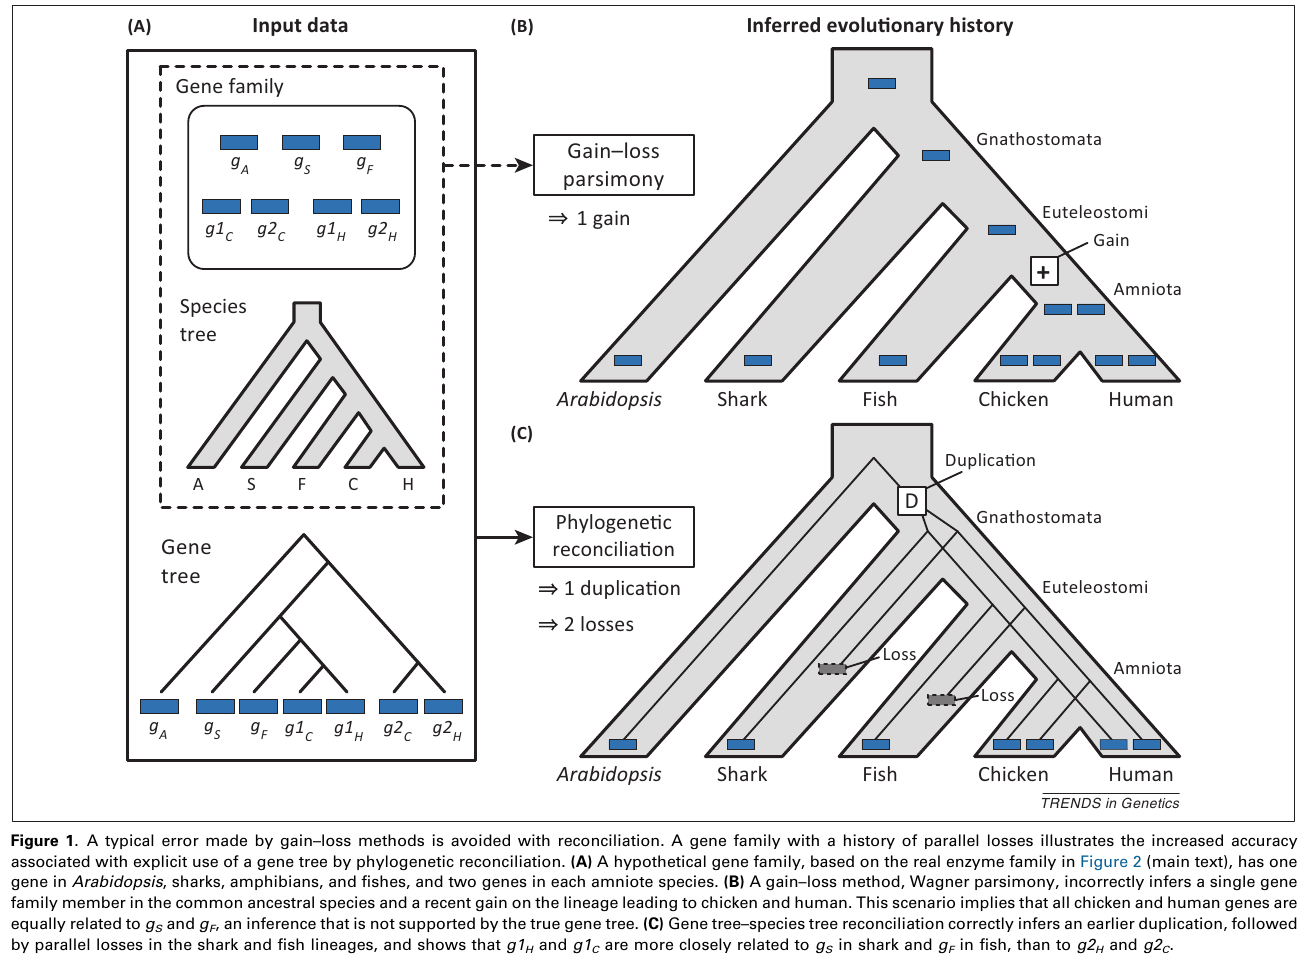
\includegraphics[width=0.9\textwidth]{capra-reconciliation-2013-fig1}
        \caption{Capra (2013) \cite{capra_how_2013}}
    \end{figure}
    \FloatBarrier

    \begin{figure}[!hbpt]
        \centering
        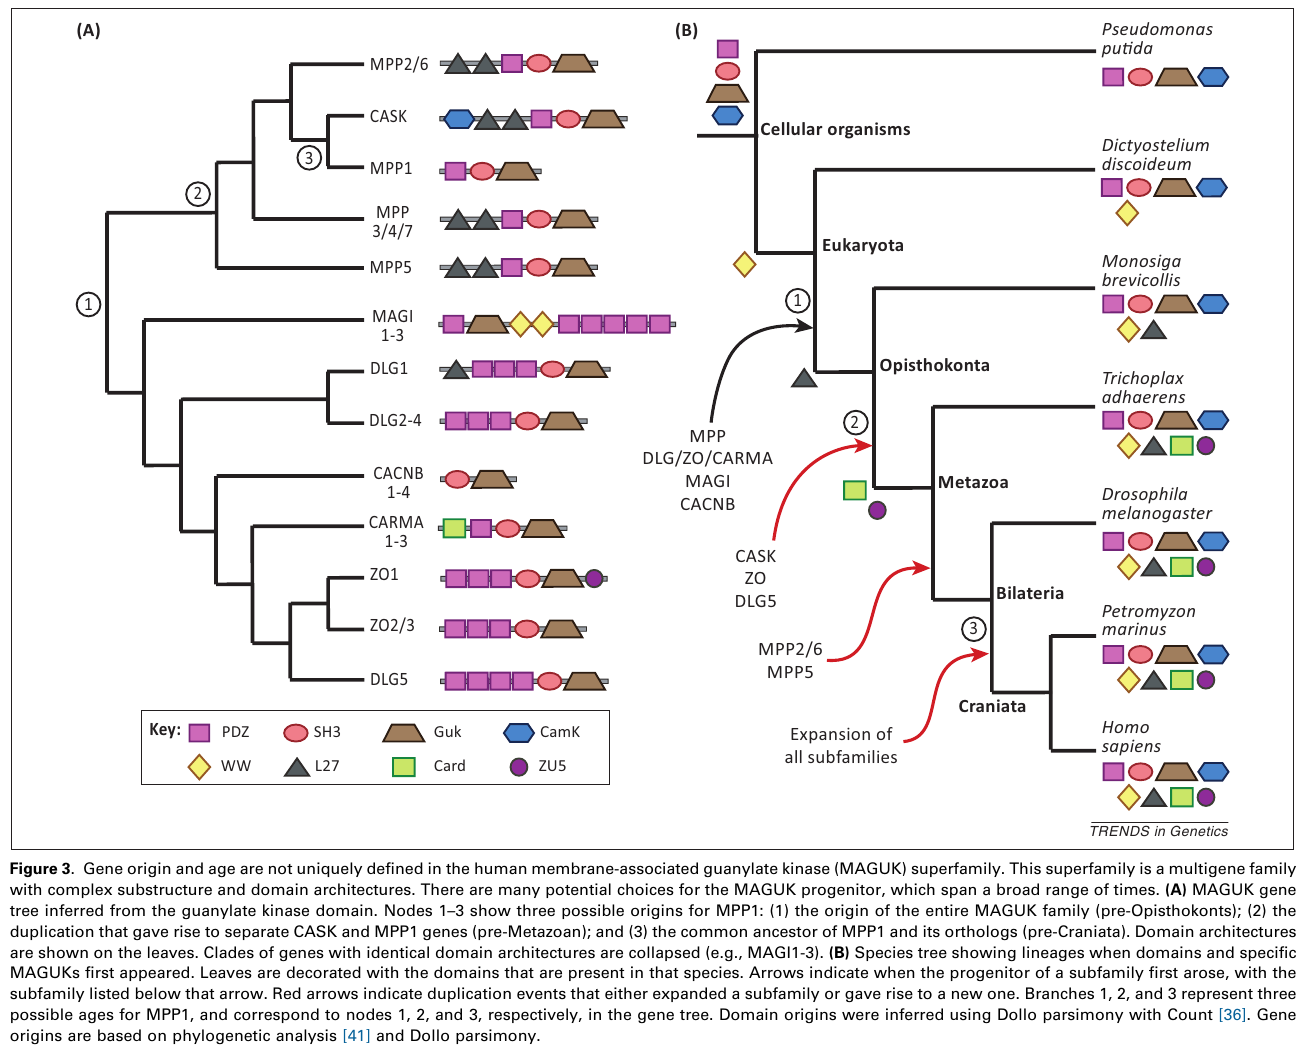
\includegraphics[width=0.9\textwidth]{capra-reconciliation-2013-fig3}
        \caption{Capra (2013) \cite{capra_how_2013}}
    \end{figure}
    \FloatBarrier

    Another problem is that major strata cannot be accurately dated

    \begin{figure}[!hbpt]
        \centering
        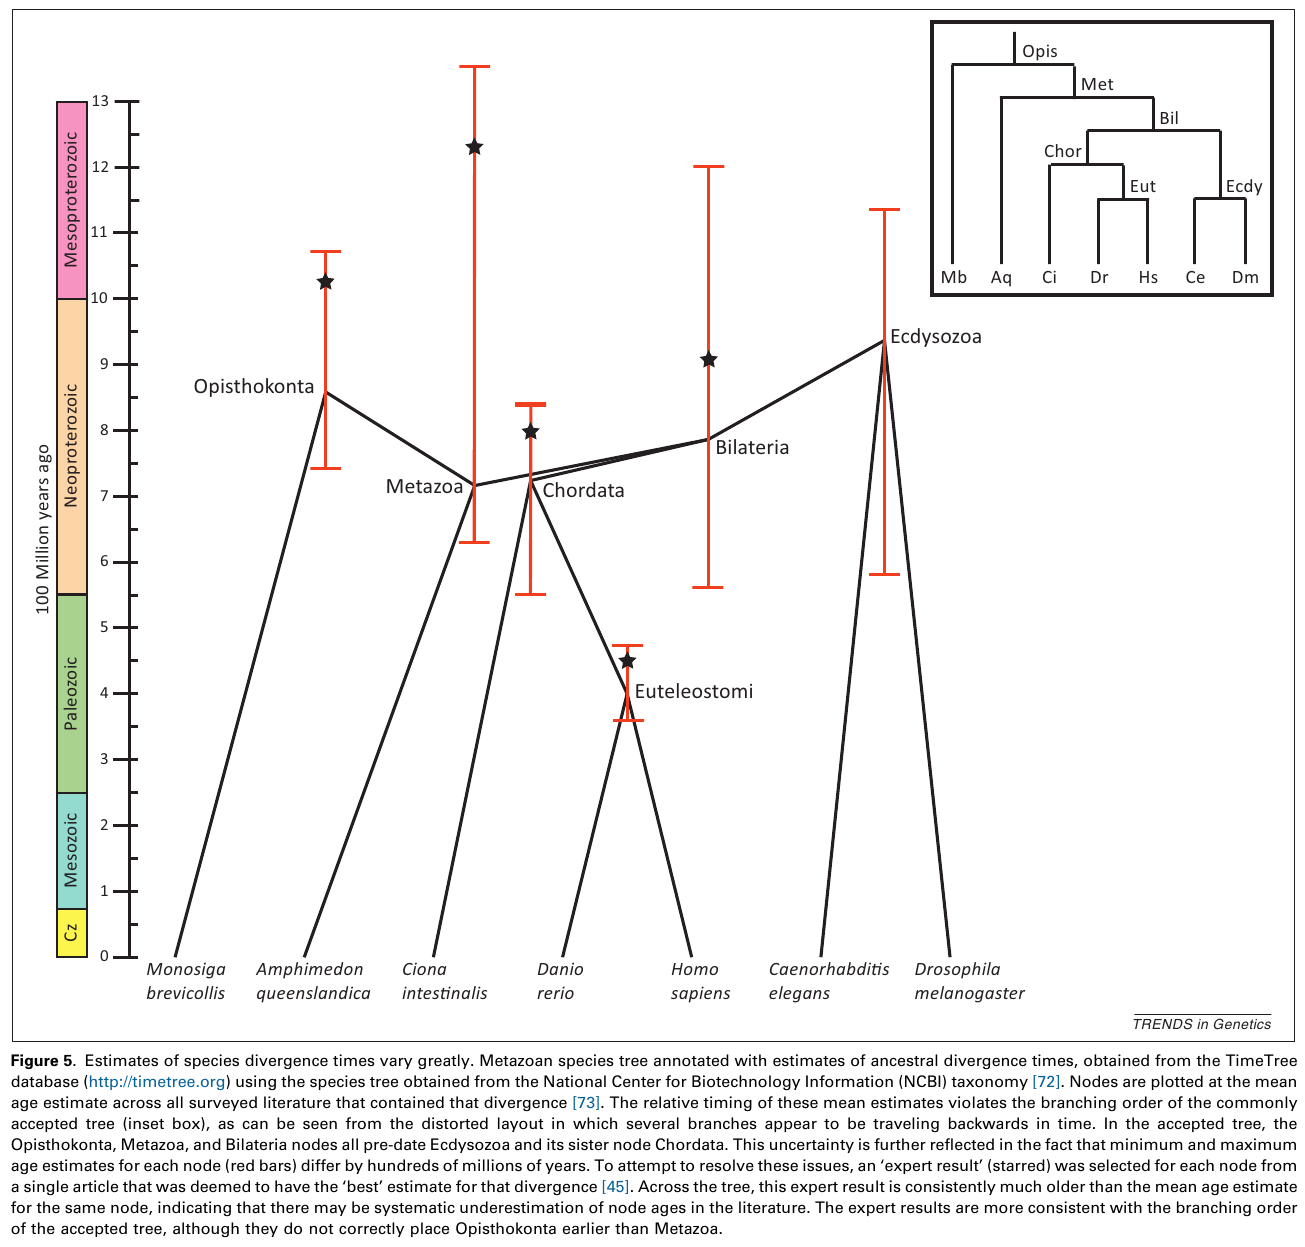
\includegraphics[width=0.9\textwidth]{capra-reconciliation-2013-fig5}
        \caption{Capra (2013) \cite{capra_how_2013}}
    \end{figure}
    \FloatBarrier

\subsection{Long (2013) New Gene Evolution: Little Did We Know}
    Citation \cite{long_new_2013}

    A very large (rather dry) review of the origins of new genes

\subsection{Lisch (2012) How important are transposons for plant evolution?}
    Citation \cite{lisch_how_2012}
    
    \begin{description}
        \item[Inactivate genes] Fairly pedestrian behavior, jump into a gene and disrupt it.
        \item[Reprogram gene expression] The simplest behvior is jumping into a
            promoter and disrupting it. However TEs have their own regulatory
            machinery, and often this can be used by the host gene. For example
            in the induction of stress regulation.
        \item[Delete, rearrange, transpose] 
        \item[Exapt coding sequence]
        \item[Epigenetics]
    \end{description}

\subsection{Bornberg-bauer (2013) Dynamics and adaptive benefits of modular
protein evolution}

    Citation \cite{bornberg-bauer_dynamics_2013}

    Claims $~80\%$ of rearangements are due to fusion, duplication and domain
    loss. The other things, exon shuffling etc, are less common.

    \begin{figure}[!hbpt]
        \centering
        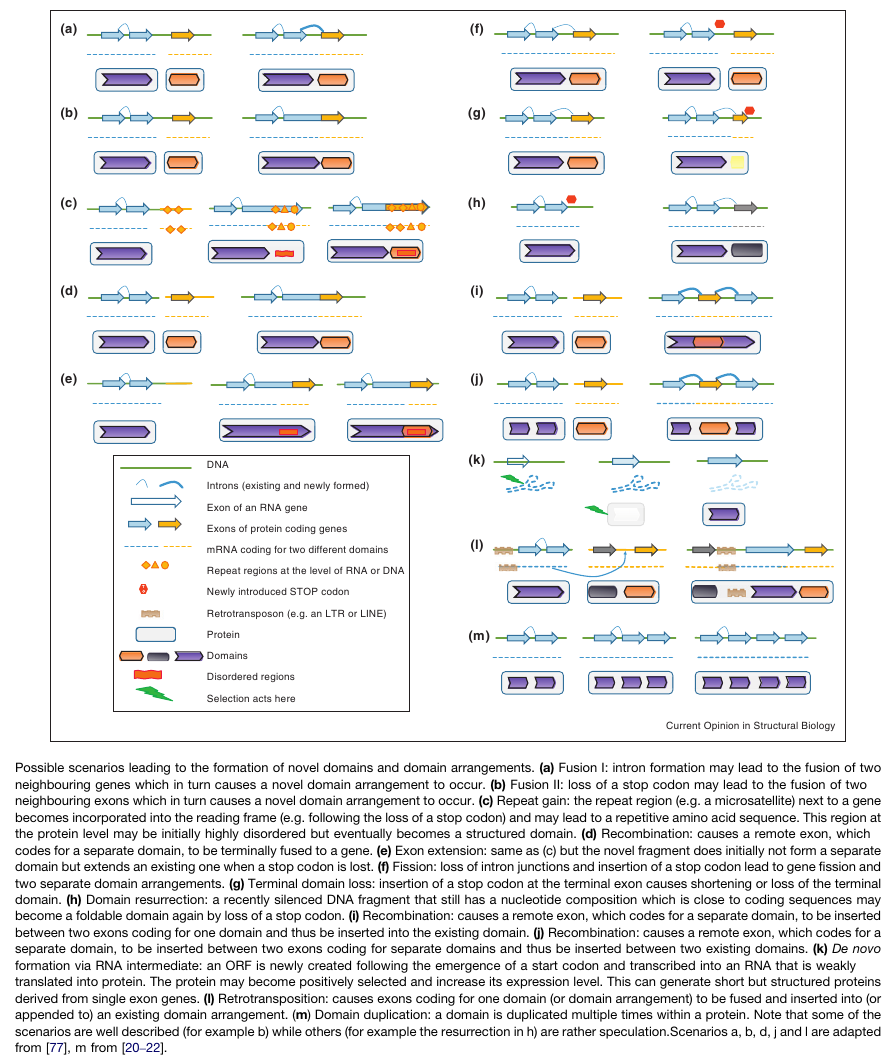
\includegraphics[height=0.7\textheight]{bornberg-bauer-2013-fig1}
        \caption{Bornberg-bauer (2013) fig1}
    \end{figure}
    \FloatBarrier

\subsection{Wu (2013) Evolution and function of de novo
originated genes}

    Citation \cite{wu_evolution_2013}

    ``Adaption following neutrality''

    Has a nice summary of the support for frequent \textit{de novo}
    proteogenesis. In both humans and drosophila, about 10\% of genes are
    \textit{de novo}.

    Mentions \textit{de novo} rise of RNAs, miRNA rise \textit{de novo} and
    by dulication at similar rates.

    States that orphans mainly rise \textit{de novo} (Khalturin et al.,
    2009; Tautz and Domazet-Loso, 2011)

    Orphan genes in animals are biased towards testes origin (many sources)

    \textit{De novo} genes are biased in humans towards brain tissue
    (several sources)

    States that little is known about function, mostly just ``guilt by
    association''.

    Neutral step then adaptive step (somewhat based off Carvunis):
\begin{enumerate}
    
    \item Neutral
    
        \begin{enumerate}
            
            \item Non-specific transcription
            \item Evolution of translateable ORF
            \item Selectable promiscuity - supported by the promiscuous
                orphan BSC4 in Sc \cite{cai_novo_2008}

        \end{enumerate}
        
    \item Adaptive
    
        \begin{enumerate}
            
            \item New gene is lifted by selection
            \item Rapid rise to importance by positive selection
        
        \end{enumerate}

\end{enumerate}

\subsection{Chen (2013) New genes as drivers of phenotypic evolution}

    Citation \cite{chen_new_2013}

    Describes the roles of orphans in metazoans.

    Keypoints: new genes rapidly gain new functions and become essential.

    New genes tend to gain roles in development, reproduction
    (spermatogenesis specifically), brain function and behaviour

    Discusses evolution of novel pathway via duplication in At (pp. 3)
    CYP98A

    New genes are needed in areas of rapid change. Resistance to stresses
    of changing environment, immune system in animals.

    Is spermatogenesis exceptional? Are there any search biases? Searching
    under streetlight?

    Artarctic fish antifreeze de novo proteins, required to deal with the
    new environment.

    ``The combination of phylostratigraphy and stage-specific gene
    expression data has revealed that the phylotypic stage expresses a
    transcriptome set representing older genes, whereas earlier and later
    developmental phases express relatively younger gene sets, in support
    of the hourglass mode \cite{kalinka_gene_2010,
    domazet-loso_phylogenetically_2010}''

    Chen doesn't mention it, but this hourglass trend has been confirmed in
    \textit{A. thaliana} as well \cite{quint_transcriptomic_2012}

    Most new essential genes are regulating early or late development.

\subsection{Ding (2012) Origins of New Genes and Evolution of Their Novel
Functions}

    Citation \cite{ding_origins_2012}
    
    Retrogenes: intronless and promoterless - pick up functions in
    spermatogenesis, courtship, ummunological response and brain

    Thought: retrogenes and orphan genes have similar functional patterns?

    ``The first straightforward search for de novo genes at the genome
    level was performed by Levine et al. (2006) in Drosophila'' pp. 9

    \textbf{Definitions of orphan genes: 1) genes without homologs 2) genes
    without homologs AND with synteny support.}

    ``Given these results together with other case studies, some common
    features of de novo genes are emerging. For example, these genes are
    relatively simple in intron/exon structure and tend to encode short and
    poorly structured proteins (Begun et al. 2006, Levine et al. 2006,
    Begun et al. 2007, Knowles \& McLysaght 2009).'' pp. 9

    There may be an ncRNA intermediate state between junk and orphan.

    ``Considering the abundance of lncRNAs in mammals and other eukaryotes
    (Mercer et al. 2009, Ponting et al. 2009), the above observations are
    particularly illuminative in suggesting the potential of lncRNAs to
    serve as a rich resource for de novo genes However, de novo genes may
    also evolve directly from noncoding DNA, as supported by the example of
    MDF1, whose orthologous loci are not expressed in the out-group species
    (Li et al. 2010b).'' pp. 10


    Chen et al. (2010) identified 566 young D. melanogaster genes that
    originated within 3–35 million years and systematically tested their
    phenotypic effects by RNA interference. Surprisingly, they found that
    30\% of these genes are essential for viability, which is comparable to
    that estimated for all genes in D. melanogaster (∼25–35\%)

\subsection{Ding (2012) Origins of New Genes and Evolution of Their Novel
Functions}

    Citation \cite{ding_origins_2012}
    
    Retrogenes: intronless and promoterless - pick up functions in
    spermatogenesis, courtship, ummunological response and brain

    Thought: retrogenes and orphan genes have similar functional patterns?

    ``The first straightforward search for de novo genes at the genome
    level was performed by Levine et al. (2006) in Drosophila'' pp. 9

    \textbf{Definitions of orphan genes: 1) genes without homologs 2) genes
    without homologs AND with synteny support.}

    ``Given these results together with other case studies, some common
    features of de novo genes are emerging. For example, these genes are
    relatively simple in intron/exon structure and tend to encode short and
    poorly structured proteins (Begun et al. 2006, Levine et al. 2006,
    Begun et al. 2007, Knowles \& McLysaght 2009).'' pp. 9

    There may be an ncRNA intermediate state between junk and orphan.

    ``Considering the abundance of lncRNAs in mammals and other eukaryotes
    (Mercer et al. 2009, Ponting et al. 2009), the above observations are
    particularly illuminative in suggesting the potential of lncRNAs to
    serve as a rich resource for de novo genes However, de novo genes may
    also evolve directly from noncoding DNA, as supported by the example of
    MDF1, whose orthologous loci are not expressed in the out-group species
    (Li et al. 2010b).'' pp. 10


    Chen et al. (2010) identified 566 young D. melanogaster genes that
    originated within 3–35 million years and systematically tested their
    phenotypic effects by RNA interference. Surprisingly, they found that
    30\% of these genes are essential for viability, which is comparable to
    that estimated for all genes in D. melanogaster (∼25–35\%)

\subsection{Khalturin (2009) More than just orphans: are
taxonomically-restricted genes important in evolution?}

    Citation \cite{khalturin_more_2009}

    A very coherent paper with a nice history or orphan genes. Covers only
    the animal side of things (with references to reasearch in bacteria).
    Focuses on cnidarian-specific genes.

    ``if the key developmental control genes are the same, and if conserved
    gene families serve similar functions in different organisms, how is
    the enormous morphological and physiological diversity within the
    animal kingdom generated?''

    Common answer: changes in regulation of these components ``rewiring''.

    \textbf{Comments on the 10-20\% orphan assertion:}

    States a 10-20\% figure for orphan composition across Eukaryota, based
    on 30 published genomes, 12 of which are Drosophilan
    \cite{clark_evolution_2007}. For some reason, he cites a 2000 paper for
    \textit{D. melanogaster} which reports 18\% or genes are orphan.
    However the 2007 paper, with the 12 genomes, reports only ~3\%. The
    genome paper suggests that many of the genes in the non-melanogaster
    genomes that were classified as being species-specific may be
    artefacts.

    Some of his other numbers I also really don't trust. Some of the
    genomes are separated by vast times (e.g. \textit{Tunicus intestinalis}
    is the sole sequenced genome in the Tunicata subphylum;
    \textit{Pristionchus pacificus} is 200 million years diverged from its
    nearest sequenced relative).
    
    His reports 11\% for rats, correctly citing the Nature rat genome paper
    \cite{gibbs_genome_2004}.  They report 10-11\% of rat proteins have no
    counterpart in humans.  \textbf{interesting sidenote:} This paper also
    says that there are 2302 rodent specific \textbf{exons} (shared in
    mouse and rat but absent in human).  Further actually the rat genome
    paper states that ``thirty-one Ensembl rat genes were collected that
    have no non-rodent homologues in current databases''. Interestingly,
    this implies a great proliferation of new genes since rats branched
    from mice, but very few of the de novo genes since the branch from
    humans have survived. As the paper says, these older de novo genes may
    have been incorporated as exons in extant genes.

    He cites a 2001 paper saying that 7\% of human genes are orphans,
    however the currnt estimate is only around 1\%.

    Overall, I really don't really trust his estimate. 

    \textbf{End of 10-20\% orphan assertion complaints}

    41 out of 50 nematocyte specific proteins are cnidarian-specific.
    \cite{hwang_evolutionary_2007}

    Basically, orphans were heavily recruited in the development of
    nematocytes. They played a role as structural componenets and
    developmental regulators.

    Most of their antimicrobial peptides show no homology. This doesn't
    really impress me. The peptides are short and necessarily change
    quickly (arms race). Aurelin is an example. Other examples exist in
    other lineages. Many very short, understudied?




\subsection{Stergiopoulos (2009) Fungal Effector Proteins}

    Citation \cite{stergiopoulos_fungal_2009}

    A voluminous review of fungal effectors. Often these effectors in fungal
    pathogens lack homology, possibly recruiting from orphans?

\subsection{Tautz (2011) The evolutionary origin of orphan genes}

    Citation \cite{tautz_evolutionary_2011}

    ``We propose that orphan genes continuously arise in any genome and
    that, at least in eukaryotes, they arise mostly through de novo
    evolution; however, we also propose that only a fraction of them
    assumes a long-term role in their respective evolutionary lineage,
    mainly in the context of evolutionary radiations'' pp. 1

    Provides rationale for trusting BLAST results. pp. 2

    Asserts gene shuffling is a minor factor citing \cite{}

\subsection{Gollery (2007) POFs: what we don’t know can hurt us}

    Citation \cite{gollery_pofs:_2007}

    Gollery phrases the issue in terms of what is unknown. He very
    specifically wants to summarize and understand the extent of our
    ignorance. The concept of POFs and PUFs are relavent to those seeking
    to delinieate the unknowneome. Orphans are differant. The orphan
    community is more interested in the novelty, the evolutionary rise,
    than the relative ignorance. Given the difference in usage, I don't
    think the terms should be merged. Gollery seeks a definition of the how
    unknown a protein is.

    While POF and orphan membership may heavily overlap, their definitions
    are quite different. POFs are defined relative to our ignorance,
    whereas orphans exist independently, being simply young genes.

    \begin{figure}[!hbpt] \centering
        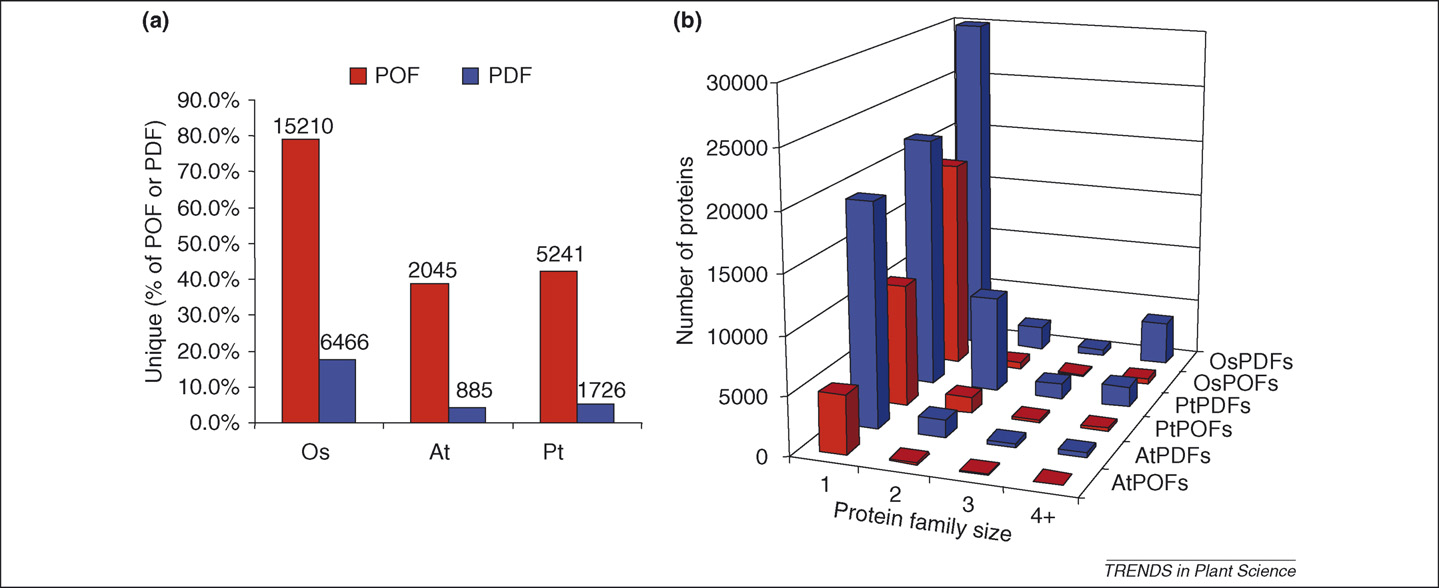
\includegraphics[scale=0.3]{gollery_hurt_2007-fig2}
        \caption{Gollery (2007) fig2} \end{figure} \FloatBarrier
